\section{Brugervejledning}

Når programmet startes via intelliJ mødes du af denne skærm:

\begin{figure}[H]
    \centering
    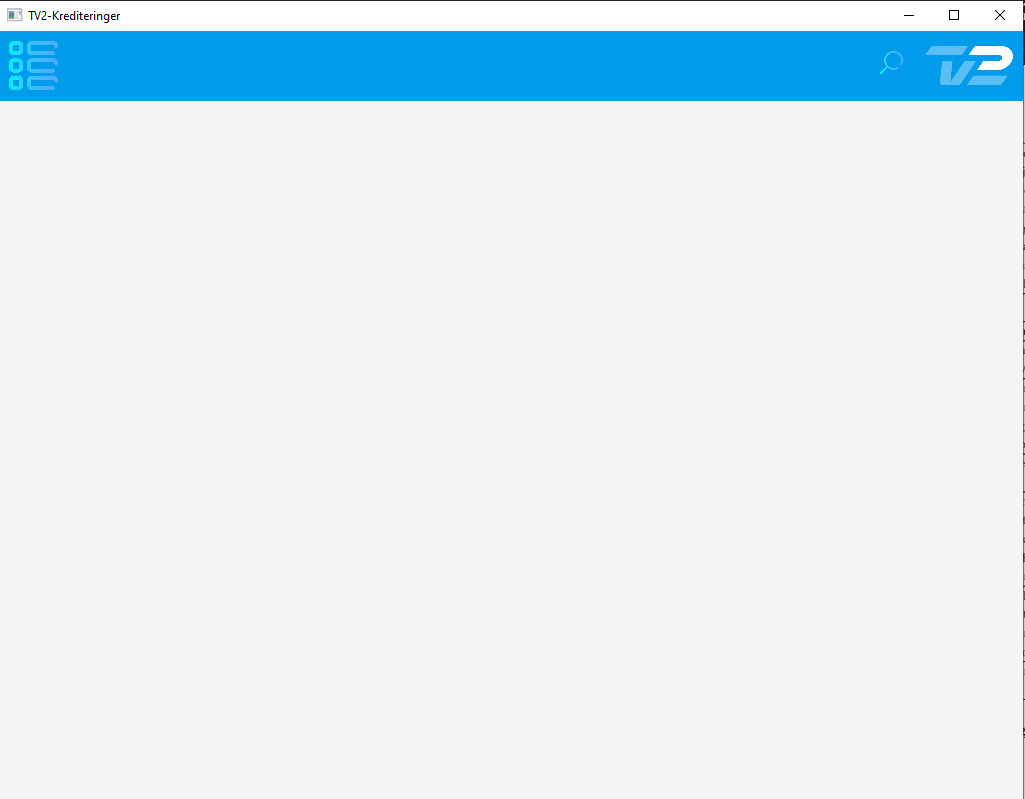
\includegraphics[scale = 0.5]{images/Home.PNG}
    \caption{Startskærm}
    \label{fig:my_label}
\end{figure}

Som standard er du ikke logget ind, og kan derfor kun foretage en søgning. For at foretage en søgning, skal du klikke til venstre for søgeknappen:

\begin{figure}[H]
    \centering
    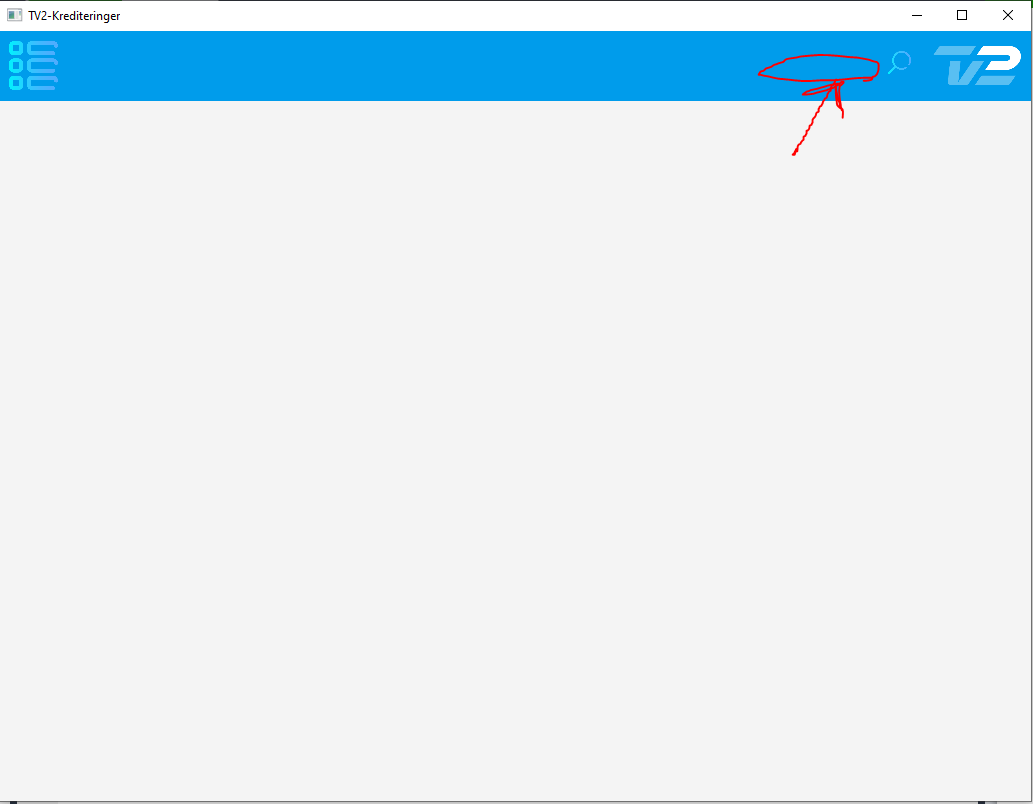
\includegraphics[scale = 0.5]{images/StartSearch.PNG}
    \caption{Start søgning}
    \label{fig:my_label}
\end{figure}

Her kan du indtaste noget tekst som du vil søge efter, og herefter trykke på forstørrelsesglasset, som vil hente alle krediteringer der svarer til teksten, og vise dig en liste.

Ønsker du at logge ind for at få muligheden for at ændre i krediteringer skal du trykke på menuen oppe til venste:

\begin{figure}[H]
    \centering
    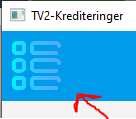
\includegraphics{images/OpenMenu.PNG}
    \caption{Åben menu}
    \label{fig:my_label}
\end{figure}

Her vælger du så Login:

\begin{figure}[H]
    \centering
    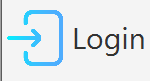
\includegraphics{images/login.PNG}
    \caption{Start Login}
    \label{fig:my_label}
\end{figure}

Og du bliver så mødt af denne skærm:

\begin{figure}[H]
    \centering
    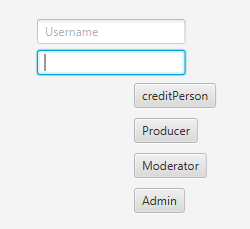
\includegraphics{images/UserTypes.PNG}
    \caption{Login skærmen}
    \label{fig:my_label}
\end{figure}

Adgangskontrollen er endnu ikke implementeret, så har anbefales at du blot vælger Admin, og så bliver du logget ind med administrator rettigheder. Du kommer nu tilbage til startskærmen, men hvis du trykke på menuen igen bliver du mødt af denne menu.

\begin{figure}[H]
    \centering
    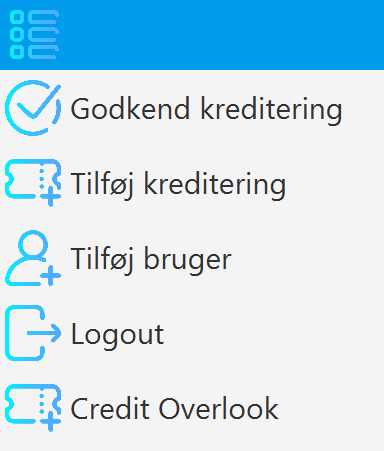
\includegraphics[scale = 0.8]{images/AdminMenu.PNG}
    \caption{Administrator menuen}
    \label{fig:my_label}
\end{figure}

Her har du adgang til alle features tilføjet i programmet. Den med avancerede er Credit Overlook, så hvis du trypper på den bliver du mødt af denne skærm:

\begin{figure}[H]
    \centering
    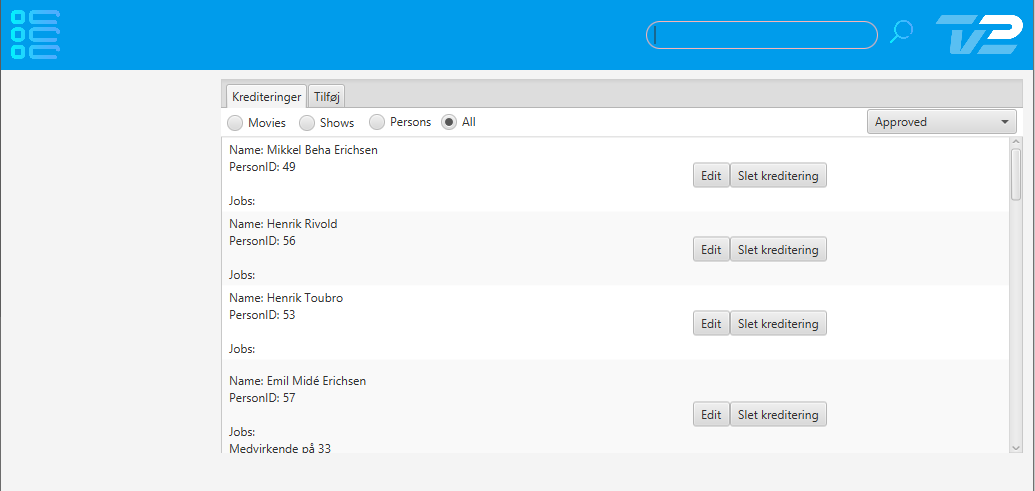
\includegraphics[scale = 0.65]{images/CreditOverlook.PNG}
    \caption{Credit overlook skærmen}
    \label{fig:my_label}
\end{figure}

Her har du nu et hav a muligheder. Øverst kan du vælge mellem "krediteringer" som viser dig alle krediteringer i systemet, som du kan sortere efter type. Eller du kan vælge tilføj, hvor du kan tilføje nye krediteringer. I toppen helt til højre kan du vælge at få vist krediteringer der er godkendt, eller venter på at blive godkendt. Da du er Admin, vil du også kunne godkende de krediteringer der ikke er godkendt. Nede ved krediteringerne Kan du vælge at trykke edit, hvor du vil kunne redigere en kreditering, eller trykke slet, som vil slette krediteringen fra databasen.